\documentclass[11pt, oneside]{article}   	% use "amsart" instead of "article" for AMSLaTeX format
\usepackage{listings}
\usepackage{geometry}                		% See geometry.pdf to learn the layout options. There are lots.
\geometry{letterpaper}                   		% ... or a4paper or a5paper or ... 
%\geometry{landscape}                		% Activate for for rotated page geometry
%\usepackage[parfill]{parskip}    		% Activate to begin paragraphs with an empty line rather than an indent
\usepackage{graphicx}				% Use pdf, png, jpg, or eps� with pdflatex; use eps in DVI mode
								% TeX will automatically convert eps --> pdf in pdflatex		
\usepackage{amssymb}
\graphicspath{{/Users/telliott_admin/Dropbox/Tex/png/}}

\title{Inverse functions}
%\author{The Author}
\date{}							% Activate to display a given date or no date

\begin{document}
\maketitle
%\section{}
%\subsection{}
\large

 For two functions $f(x)$ and $g(x)$, we say that $f$ and $g$ are inverse functions if application of first g and then f in series, called the composition of $f$ and $g$, gives $x$ back again.  The converse is also true if $f$ and $g$ are inverses.  Sometimes there are restrictions on the domain for one function but not the other.
 \[ f \circ g  (x) = f(\ g(x)) \ = g(\ f(x)) = g \circ f  (x) \]
 
 Some simple examples are
 \[ f(x) = x + 1, \ \ \ \ g(x) = x - 1 \]
 \[ f(x) = cx, \ \ \ \ g(x) = \frac{1}{c}x \]
 
Familiarity with analytical geometry will be enough to recognize that the product of the slopes of f and g is equal to 1 for these first two equations, at least.  This statement that slopes of inverse functions are multiplicative inverses hides a subtle difficulty, however.
 
For example, what about
 \[ f(x) = x^2, \ \ \ \ g(x) = \sqrt{x} \]
 \[ f'(x) = 2x, \ \ \ \ g'(x) = \frac{1}{2 \sqrt{x}}, \ \ \ \ \  2x \ \frac{1}{2 \sqrt{x}} \neq 1 \]
Or 
\[ f(x) = e^x, \ \ \ \ g(x) = ln(x) \]
\[ e^{ln(x)} = x, \ \ \ \  ln(e^x) = x \]
But
 \[ f'(x) = e^x, \ \ \ \ g'(x) = \frac{1}{x}, \ \ \ \ \  e^x \ \frac{1}{x} \neq 1 \]
Still, a quick graph looks like these functions are symmetric about y = x.
\begin{center}
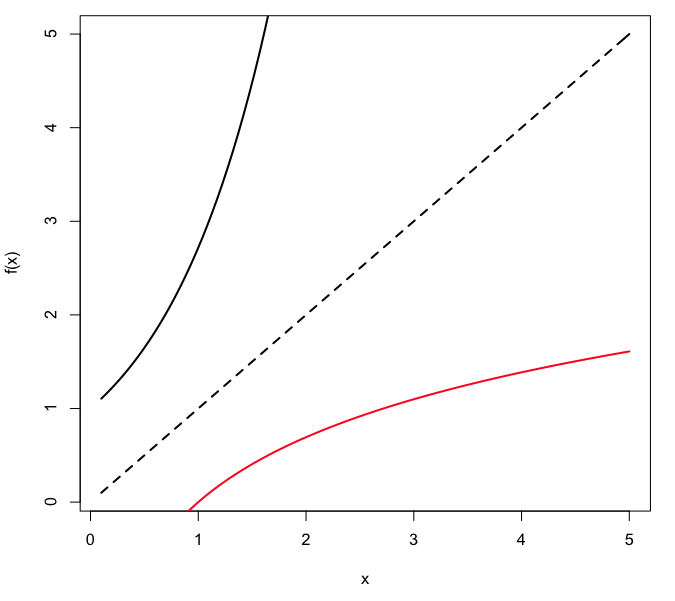
\includegraphics [scale=0.3] {log_v_e.png}
\end{center}
The R code was
\small
\begin{lstlisting}
f <- function(x) { x }
x1 = 0.1
x2 = 5
plot(f,from=x1,to=x2, col='black',lwd=2,lty=2)
plot(log,from = x1,to = x2,col='red', lwd=2,add = T)
plot(exp,from = x1,to = x2,col='black', lwd=2,add = T)
\end{lstlisting}
\large

But as we saw above, the slopes do not multiply to give 1, and the symmetry about $y = x$ is close but not exactly right.  There is something else going on.

What is happening is that although we've written $f(x)$ and $g(x)$ as functions of $x$, which is perfectly valid, when we are composing to apply the inverse after the forward operation we need to write something slightly different:
\[ y = f(x), \ \ \ \  x = g(y) \]
So, when we multiply the slopes together to test equality with 1, we must evaluate the expressions for different inputs!  Going back to the square root
 \[ f'(x) = 2x, \ \ \ \ g'(y) = \frac{1}{2 \sqrt{y}} \]
 If we evaluate $f(x) = x^2$ at $x=5$ and obtain a slope of $f'(x) = 2x=10$, we must evaluate $g'(y)$ at 25, then we have $g'(y) = 1/(2 \sqrt{25}) $ and obtain the correct result.
Similarly, for 
 \[ f'(x) = e^x, \ \ \ \ g'(y) = \frac{1}{y} \]
if we evaluate $f(x)=e^x$ at $x=2$ we obtain a slope of $e^2$;  we must evaluate $g'(y)$ at $y=e^2$ giving slope $= 1/e^2$. Then the two slopes together give 1.
\end{document}  